% !TEX root =  ../supplementary.tex
\section{Personalized Biopsies Based on Risk of GS7}
Consider some real patients from the PRIAS database shown in Figure~\ref{fig:demo_pat1_supp} to Figure~\ref{fig:demo_pat4_supp}. We intend to develop personalized schedule of biopsies for these patients. Using the joint model fitted to the PRIAS dataset, we first obtain their cumulative risk of GS7 over the entire follow-up period (see Equation~(\ref{eq:dynamic_risk_prob}). This cumulative risk accounts for their entire history of PSA as well as the time of their latest negative biopsy. For a new patient $j$ we suggest a personalized risk based biopsy if their cumulative risk of GS7 $R_j(s \mid t, s)$  at their current visit $s$, given the time of their latest negative biopsy $t$, is above a certain threshold (e.g., 10\% risk). Suppose that in this way a decision of biopsy is taken at time $s$. Since patients may be removed from AS upon detection of GS7, subsequent biopsies are scheduled assuming we do not detect GS7 at time $s$. Thus, at the next visit at time $s + 1$, the time of the latest negative biopsy is updated to time $s$. The updated cumulative risk of GS7 at time $s + 1$ is then $R_j(s + 1 \mid s, s)$. If $R_j(s + 1 \mid s, s) < 10\%$, then we decide for a biopsy at time $s + 2$ using the threshold $R_j(s + 2 \mid s,s)$. On the other hand if $R_j(s + 1 \mid s, s) \geq 10\%$ then then we decide for a biopsy at time $s + 2$ using the threshold $R_j(s + 2 \mid s + 1, s)$. While scheduling these biopsies we always maintain a minimum gap of one year. Personalized schedules can also be made with any other risk threshold such as 5\% or 15\%.

To assist patients in making an informed choice for a schedule, be it personalized or fixed, we provide them patient-specific consequences of following each schedule. To this end, we first calculate the probability of occurrence of GS7 between successive biopsies of each schedule. Using these probabilities we then obtain the expected delay in detection of GS7 for following that schedule. Thus, patients have a method to compare across various schedules in terms of the personalized burden (time and total biopsies), and personalized benefit (less delay in detection of GS7 is beneficial). Suppose once again that for patient $j$, the time of latest negative biopsy is $t$, and current visit time is $s > t$. Then equation for the expected delay $D_j(\mathcal{S} \mid t,s)$ in detection of GS7 using schedule of biopsies $\mathcal{S} = \{t_1, \ldots, t_h\}$, where $t_1 \geq s$, and $t_h$ is the horizon time up to which we want to schedule biopsies, is given by:
\begin{equation}
\label{eq:expected_delay}
\begin{split}
D_j(\mathcal{S} \mid t,s) &= \sum_{v=1}^{h-1} \Big\{R_j(t_{v+1}\mid t,s) - R_j(t_v\mid t,s)\Big\} \\ & \times  \Bigg\{t_{v+1} - t_{v} - \int_{t_v}^{t_{v+1}} \frac{R_j(t_{v+1}\mid t,s)-R_j(u \mid t,s)}{R_j(t_{v+1}\mid t,s) - R_j(t_v\mid t,s)} \mathrm{d}u \Bigg\}
\end{split}
\end{equation}
 
The personalized and fixed schedules, and their consequences for a few real patients from the PRIAS dataset are shown in Figure~\ref{fig:demo_pat1_supp} to Figure~\ref{fig:demo_pat4_supp}. 

\begin{figure}
\centerline{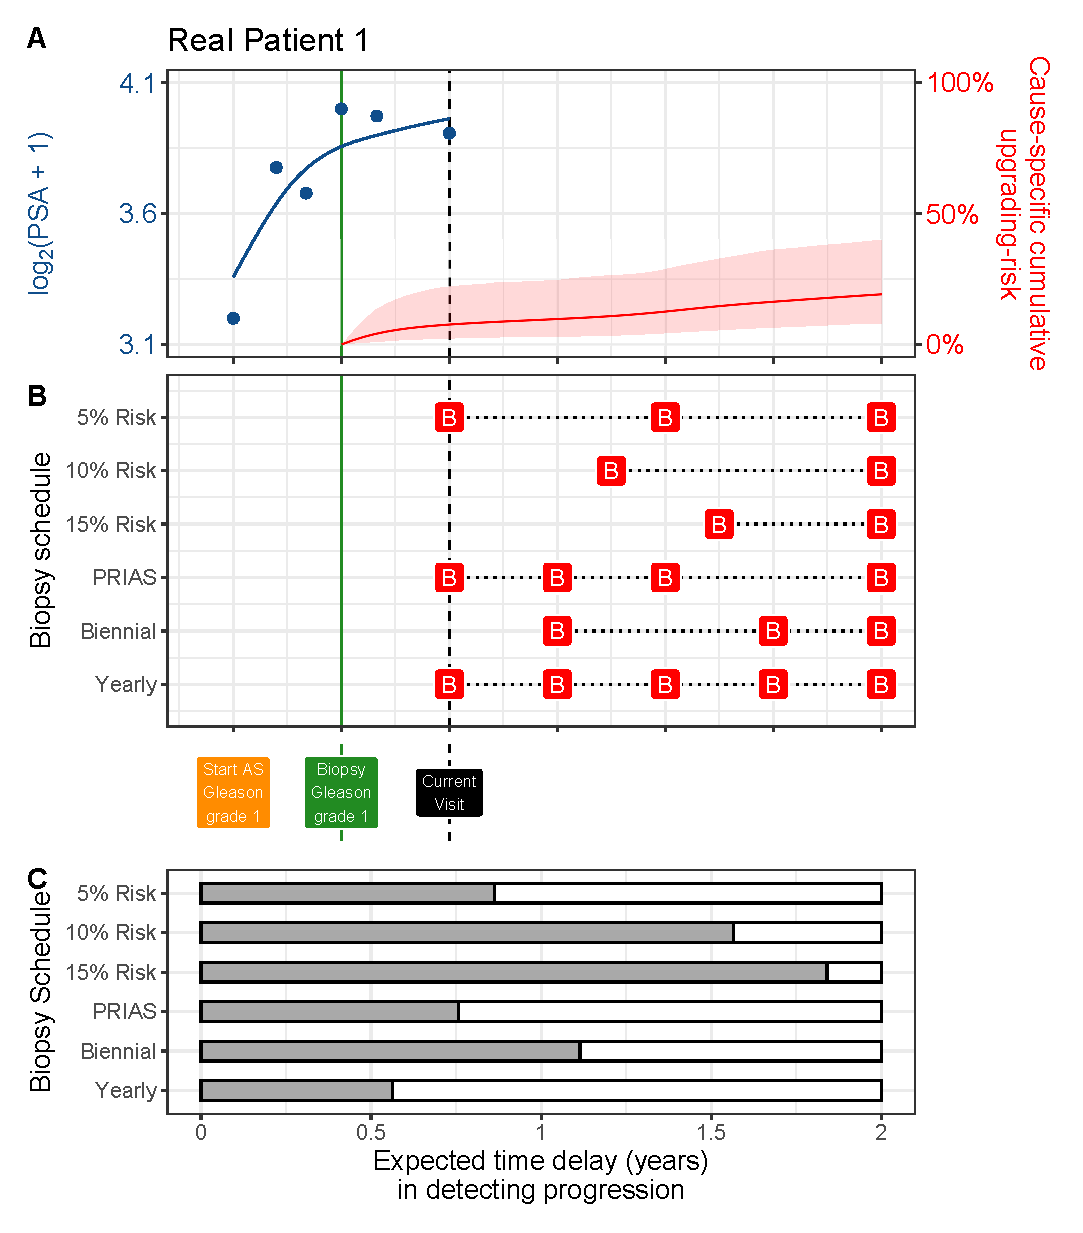
\includegraphics[width=\columnwidth]{images/demo_pat1_supp.eps}}
\caption{\textbf{Personalized and fixed schedules of biopsies patient 1}. \textbf{Panel~A:} shows the observed and fitted $\log_2(\mbox{PSA} + 1)$ measurements (Equation~\ref{eq:long_model_psa}), and the dynamic cumulative risk of Gleason $\geq$ 7 (see \ref{sec:param_estimates_jm_fit_prias}) over follow-up period. \textbf{Panel~B} shows the personalized and fixed schedules of biopsies with a `B' indicating times of biopsies. In the bottom two panels, the various schedules are compared in terms of the number of biopsies they schedule, and the expected delay in detection of Gleason $\geq$ 7 if they are followed.}
\label{fig:demo_pat1_supp}
\end{figure}

\begin{figure}
\centerline{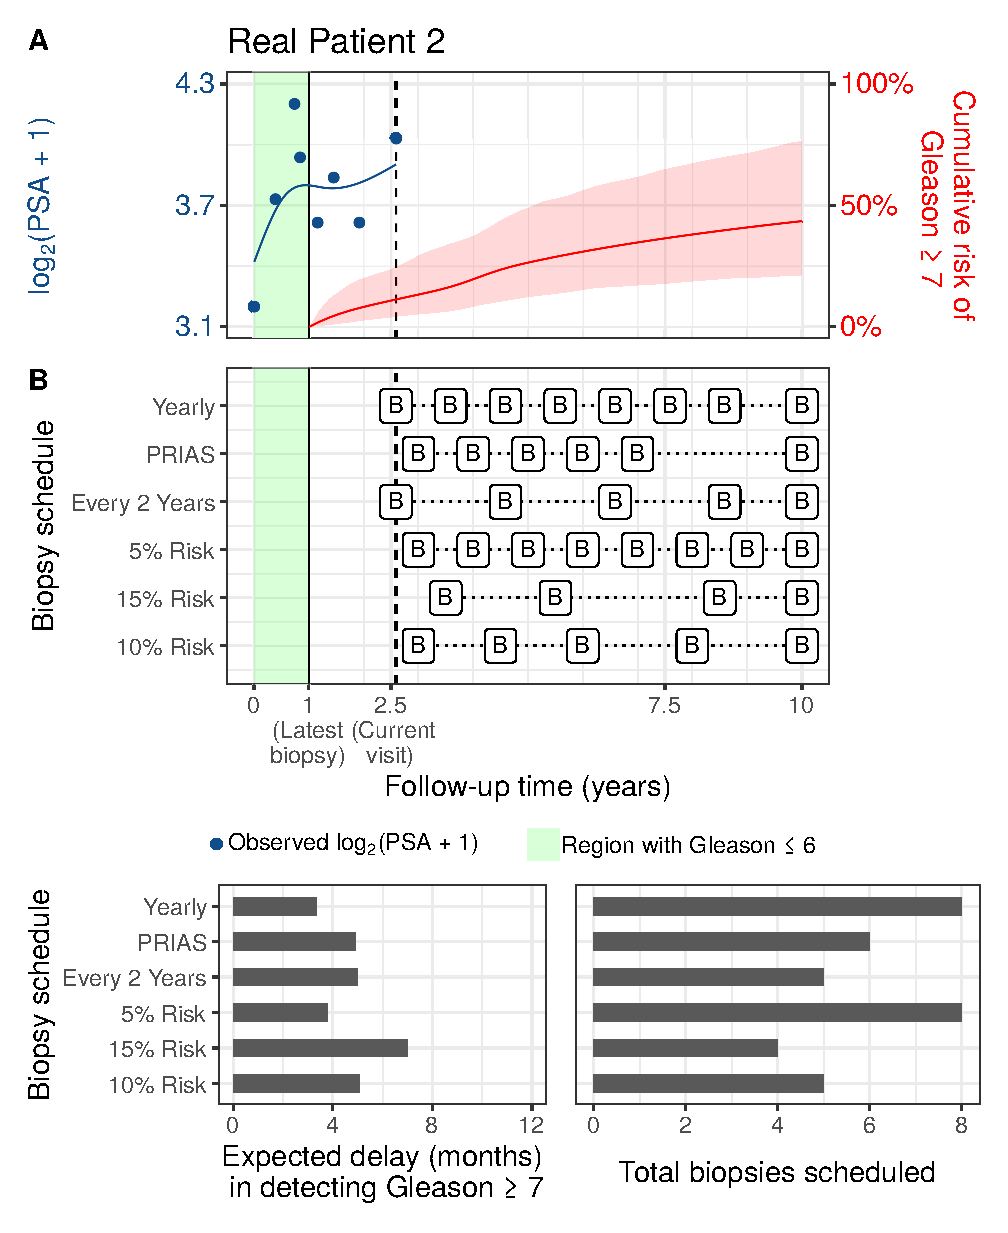
\includegraphics[width=\columnwidth]{images/demo_pat2_supp.eps}}
\caption{\textbf{Personalized and fixed schedules of biopsies patient 2}. \textbf{Panel~A:} shows the observed and fitted $\log_2(\mbox{PSA} + 1)$ measurements (Equation~\ref{eq:long_model_psa}), and the dynamic cumulative risk of Gleason $\geq$ 7 (see \ref{sec:param_estimates_jm_fit_prias}) over follow-up period. \textbf{Panel~B} shows the personalized and fixed schedules of biopsies with a `B' indicating times of biopsies. In the bottom two panels, the various schedules are compared in terms of the number of biopsies they schedule, and the expected delay in detection of Gleason $\geq$ 7 if they are followed.}
\label{fig:demo_pat2_supp}
\end{figure}

\begin{figure}
\centerline{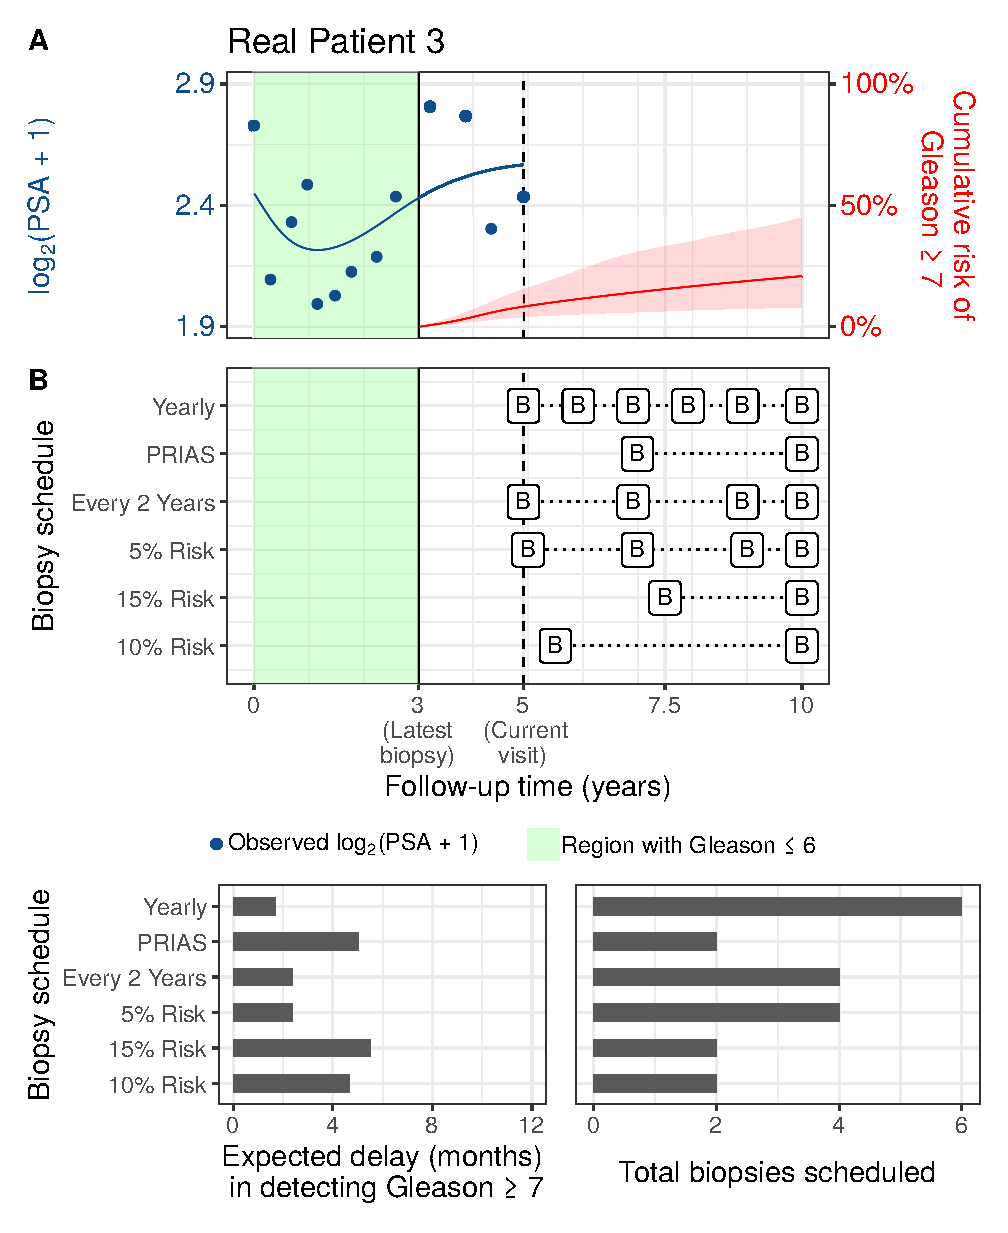
\includegraphics[width=\columnwidth]{images/demo_pat3_supp.eps}}
\caption{\textbf{Personalized and fixed schedules of biopsies patient 3}. \textbf{Panel~A:} shows the observed and fitted $\log_2(\mbox{PSA} + 1)$ measurements (Equation~\ref{eq:long_model_psa}), and the dynamic cumulative risk of Gleason $\geq$ 7 (see \ref{sec:param_estimates_jm_fit_prias}) over follow-up period. \textbf{Panel~B} shows the personalized and fixed schedules of biopsies with a `B' indicating times of biopsies. In the bottom two panels, the various schedules are compared in terms of the number of biopsies they schedule, and the expected delay in detection of Gleason $\geq$ 7 if they are followed.}
\label{fig:demo_pat3_supp}
\end{figure}

\begin{figure}
\centerline{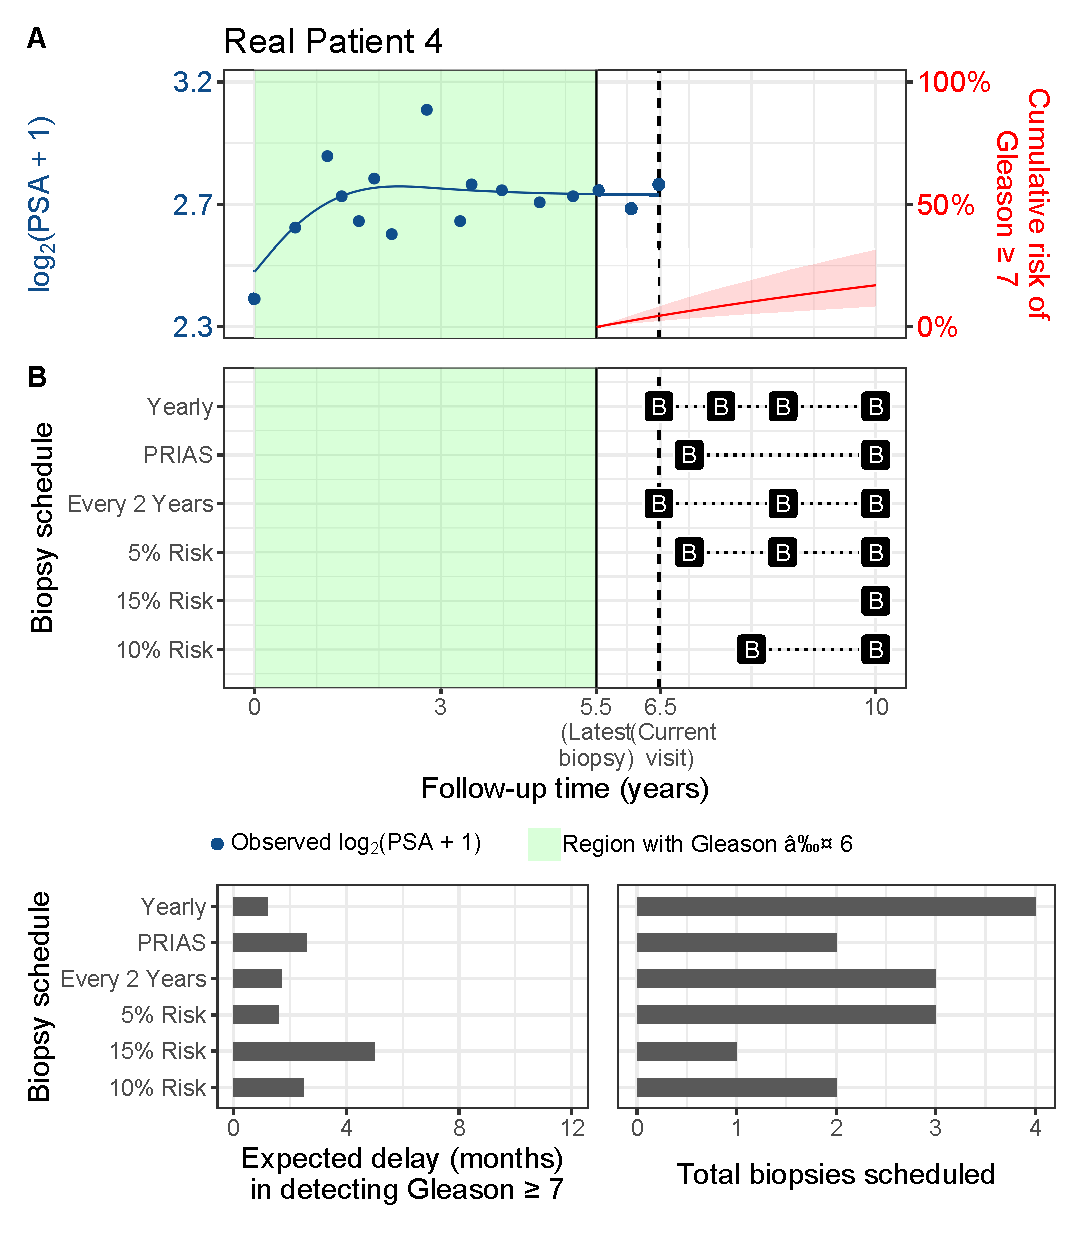
\includegraphics[width=\columnwidth]{images/demo_pat4_supp.eps}}
\caption{\textbf{Personalized and fixed schedules of biopsies patient 4}. \textbf{Panel~A:} shows the observed and fitted $\log_2(\mbox{PSA} + 1)$ measurements (Equation~\ref{eq:long_model_psa}), and the dynamic cumulative risk of Gleason $\geq$ 7 (see \ref{sec:param_estimates_jm_fit_prias}) over follow-up period. \textbf{Panel~B} shows the personalized and fixed schedules of biopsies with a `B' indicating times of biopsies. In the bottom two panels, the various schedules are compared in terms of the number of biopsies they schedule, and the expected delay in detection of Gleason $\geq$ 7 if they are followed.}
\label{fig:demo_pat4_supp}
\end{figure}